\PassOptionsToPackage{svgnames}{xcolor} % permet d'éviter le clash du package xcolor (chargé avec documentclass avec l'option [])

\documentclass[a4paper]{article}
\usepackage[utf8]{inputenc}
\usepackage{amsmath}
\usepackage[french]{babel}
\usepackage[T1]{fontenc}
\usepackage{amsfonts}
\usepackage{amssymb}
\usepackage[usenames, dvipsnames, svgnames, table]{colortbl}
\usepackage{hyperref}
\usepackage{tikz}
\usepackage{fancyvrb}
\usepackage{booktabs}
\usepackage{graphicx}
\usepackage{pgfsys}
\usepackage{keyval}
\usepackage{subfig}
\usepackage{multicol}
\usepackage{tabularx}
\usepackage{array}
\usepackage{float}
\usepackage{helvet}
\usepackage{xifthen}
\renewcommand{\familydefault}{\sfdefault}
% \usepackage{placeins} % gestion des flottants
\usepackage[justification = centering]{caption}
\usepackage{enumitem}
\usepackage[section]{placeins}
% \usepackage{subcaption}
\usepackage{subfig}
\usepackage{multirow}
% \usepackage[output-decimal-marker = {, }]{siunitx}
\usepackage[autolanguage]{numprint}
\usepackage{titlesec}

\captionsetup{width = 9cm}

% Format des titres
\titleformat{\section}[frame]{\normalfont}{\filright\footnotesize\enspace SECTION \thesection\enspace}{8pt}{\Large\bfseries\filcenter}
\titleformat{\subsection}{\normalfont}{\hspace{0em}\large\bfseries\thesubsection}{8pt}{\large\bfseries}
\titleformat{\subsubsection}{\normalfont}{\hspace{5em}\normalsize\bfseries\thesubsubsection}{8pt}{\normalsize\bfseries}
\titleformat{\paragraph}{\normalfont}{\hspace{2em}\normalsize\underline\theparagraph}{3pt}{\normalsize\underline}

% Mise en page
\voffset -2cm
\hoffset 0cm
\oddsidemargin 0cm
\evensidemargin -0.5cm
\textwidth 17cm
\topmargin 1cm
\textheight 25cm
\parindent 0cm
\columnsep 0.7cm

% Définition des types des colonnes (tableaux)
\newcolumntype{P}[1]{>{\centering\arraybackslash}p{#1}}
\newcolumntype{M}[1]{>{\centering\arraybackslash}m{#1}}
\newcolumntype{C}{>{\centering\arraybackslash}c}

% ---------- Gestion des figures sur des pages vides (apparaissaient au milieu de la page)
\makeatletter% Set distance from top of page to first float
\setlength{\@fptop}{5pt}
\makeatother

% ----- Modification du nom des tableaux/figures
\addto\captionsfrench{\def\tablename{\footnotesize Tableau}}
\addto\captionsfrench{\def\figurename{\footnotesize Figure}}

% ----- Réglages des espaces entre floats
\setlength{\textfloatsep}{0.2cm plus 0.1cm minus 0.1cm} % 0.25
\setlength{\floatsep}{0.2cm plus 0.1cm minus 0.1cm}
\setlength{\intextsep}{0.2cm plus 0.1cm minus 0.1cm}
% \intextsep

% ----- Réglages sur la part de texte, le déplacement des floats aux pages suivantes etc...
\renewcommand{\textfraction}{0.05}
\renewcommand{\topfraction}{0.8}
\renewcommand{\bottomfraction}{0.8}
\renewcommand{\floatpagefraction}{0.75}

\setcounter{tocdepth}{2}     % Dans la table des matieres
\setcounter{secnumdepth}{2}  % Avec un numero.

% Commande édition conditionnelle
\newcommand{\EditIf}[4]{
\ifthenelse{
\equal{#1}{#2}
}{#3}{#4}
}









\begin{document}
\textcolor{red}{\Large ATTENTION checl de EssReg à revoir}

% -- 1st page
\thispagestyle{empty} % la page en tour n'a pas de numéro de page

\begin{center}

\begin{figure}[ht]
\centering


\includegraphics[height = 2.5cm]{/Users/Valentin/Travail/Outils/GitHub/PermGF-ShinyApp/data/images/logos/logo_ForestAllia_2.png}
\end{figure}

\vspace*{5cm}
\textbf{Rapport automatique de vérification des données GF de la forêt\\
\vspace{0,5cm}
Forêt Communale d'Onex}\\
\vspace{1cm}
\vspace{0,5cm}
\date{\year}
\end{center}

\begin{center}
\today\\
% \vspace{15cm}
\vfill


\begin{multicols}{3}
\begin{flushleft}

\includegraphics[height = 1.5cm]{/Users/Valentin/Travail/Outils/GitHub/PermGF-ShinyApp/data/images/logos/AFI_logo.jpg}
\end{flushleft}

\scriptsize{Conçu et développé par\\ Max Bruciamacchie et Valentin Demets\\ en collaboration avec Julien Tomasini}

\begin{flushright}

\includegraphics[height = 1.5cm]{/Users/Valentin/Travail/Outils/GitHub/PermGF-ShinyApp/data/images/logos/APT_LOGO.png} % changement
\end{flushright}
\end{multicols}

\end{center}
% -- fin 1st page

\newpage\null\thispagestyle{empty}\newpage

\section*{Introduction}
Que ce soit à l'échelle d'une propriété, d'un massif ou d'un territoire, un réseau de placettes permanentes fournit aux décideurs les éléments nécessaires à des audits réguliers des espaces forestiers dont ils sont maîtres d'ouvrage, et il sert aux gestionnaires à optimiser la gestion qu'ils sont chargés de mettre en \oe uvre.\\
Ce rapport présente de manière succincte l'état de complétude et de validation des données pour la forêt Forêt Communale d'Onex (fichier source : 23-Forêt Communale d'Onex.xlsx). Il est généré automatiquement grâce au logiciel RStudio.


\tableofcontents
\thispagestyle{empty} % la page en tour n'a pas de numéro de page
\setcounter{page}{0}
\newpage

\section{Tables principales/administrateur}
\subsection{Table Foret}
\subsubsection{Contrôle des valeurs vides}
\paragraph{Variables indispensables à l'analyse des données}
\textcolor{ForestGreen}{\textbf{Vérifié}} - Il n'y a aucune valeur vide dans les variables indispensables à l'analyse des données (NumForet) de la table 'Forets'. \\ 

\paragraph{Variables non indispensables à l'analyse des données}
\textcolor{blue}{\textbf{Remarque}} - Il manque des informations (vides) dans la table 'Forets' pour les variables Nom, Proprietaire, Gestionnaire, SurfForet. \\ 

% latex table generated in R 4.4.2 by xtable 1.8-4 package
% Fri Nov 29 17:15:39 2024
\begin{table}[ht]
\centering
\begingroup\scriptsize
\begin{tabular}{|M{2cm}|M{1cm}|}
  \hline
Colonne & Nombre de vides \\ 
  \hline
Gestionnaire & 1 \\ 
   \hline
Proprietaire & 1 \\ 
   \hline
\end{tabular}
\endgroup
\caption{\footnotesize{Vides constatés dans les variables Nom, Proprietaire, Gestionnaire, SurfForet, non indispensables à l'analyse des données}} 
\label{Forets-missing_values_for_non_essential_vars}
\end{table}
\FloatBarrier
\subsubsection{Contrôle des valeurs dupliquées}
\paragraph{Variables indispensables à l'analyse des données}
\textcolor{ForestGreen}{\textbf{Vérifié}} - Il n'y a aucun doublon détecté dans les variables indispensables à l'analyse des données (NumForet) de la table 'Forets'. \\ 

\paragraph{Variables non indispensables à l'analyse des données}
\textcolor{ForestGreen}{\textbf{Vérifié}} - Il n'y a aucun doublon détecté dans les variables non indispensables à l'analyse des données (Nom, Proprietaire, Gestionnaire, SurfForet) de la table 'Forets'. \\ 

\begin{center}
\textcolor{Blue}{\textbf{La table peut contenir des irrégularités (cf remarques)}}
\end{center}


\FloatBarrier

\subsection{Table Cycle}
\subsubsection{Contrôle des valeurs vides}
\paragraph{Variables indispensables à l'analyse des données}
\textcolor{ForestGreen}{\textbf{Vérifié}} - Il n'y a aucune valeur vide dans les variables indispensables à l'analyse des données (NumForet, Cycle, Annee) de la table 'Cycles'. \\ 

\paragraph{Variables non indispensables à l'analyse des données}
\textcolor{blue}{\textbf{Remarque}} - Il manque des informations (vides) dans la table 'Cycles' pour les variables Date, Operateurs, Financeurs. \\ 

% latex table generated in R 4.4.2 by xtable 1.8-4 package
% Fri Nov 29 17:15:39 2024
\begin{table}[ht]
\centering
\begingroup\scriptsize
\begin{tabular}{|M{2cm}|M{1cm}|}
  \hline
Colonne & Nombre de vides \\ 
  \hline
Financeurs & 1 \\ 
   \hline
\end{tabular}
\endgroup
\caption{\footnotesize{Vides constatés dans les variables Date, Operateurs, Financeurs, non indispensables à l'analyse des données}} 
\label{Cycles-missing_values_for_non_essential_vars}
\end{table}
\FloatBarrier
\subsubsection{Contrôle des valeurs dupliquées}
\paragraph{Variables indispensables à l'analyse des données}
\textcolor{ForestGreen}{\textbf{Vérifié}} - Il n'y a aucun doublon détecté dans les variables indispensables à l'analyse des données (NumForet, Cycle, Annee) de la table 'Cycles'. \\ 

\paragraph{Variables non indispensables à l'analyse des données}
\textcolor{ForestGreen}{\textbf{Vérifié}} - Il n'y a aucun doublon détecté dans les variables non indispensables à l'analyse des données (Date, Operateurs, Financeurs) de la table 'Cycles'. \\ 

\subsubsection{Contrôle sur les numéros d'inventaire (cycles) rencontrés dans les tables d'inventaire}
Principe : tous les cycles rencontrées dans l'inventaire doivent figurer dans la table Cycles\\ 
\paragraph{Cycles de la table Arbres}
\textcolor{ForestGreen}{\textbf{Vérifié}} - Tous les cycles d'inventaire de la table 'Arbres' sont présents dans la table 'Cycles'. \\ 

\paragraph{Cycles de la table Reges}
\textcolor{ForestGreen}{\textbf{Vérifié}} - Tous les cycles d'inventaire de la table 'Reges' sont présents dans la table 'Cycles'. \\ 

\paragraph{Cycles de la table Cercles}
\textcolor{ForestGreen}{\textbf{Vérifié}} - Tous les cycles d'inventaire de la table 'Cercles' sont présents dans la table 'Cycles'. \\ 

\paragraph{Cycles de la table BMSLineaires}
\textcolor{ForestGreen}{\textbf{Vérifié}} - Tous les cycles d'inventaire de la table 'BMSLineaires' sont présents dans la table 'Cycles'. \\ 

\paragraph{Cycles de la table BMSCercles}
\textcolor{ForestGreen}{\textbf{Vérifié}} - Tous les cycles d'inventaire de la table 'BMSCercles' sont présents dans la table 'Cycles'. \\ 

\begin{center}
\textcolor{Blue}{\textbf{La table peut contenir des irrégularités (cf remarques)}}
\end{center}


\FloatBarrier

\subsection{Table Echantillonnage}
\subsubsection{Contrôle des valeurs vides}
\paragraph{Variables indispensables à l'analyse des données}
\textcolor{ForestGreen}{\textbf{Vérifié}} - Il n'y a aucune valeur vide dans les variables indispensables à l'analyse des données (NumForet, Cycle, Strate) de la table 'Echantillonnages'. \\ 

\paragraph{Variables non indispensables à l'analyse des données}
\textcolor{blue}{\textbf{Remarque}} - Il manque des informations (vides) dans la table 'Echantillonnages' pour les variables Surface, NbPlac, DiamLim1, Rayon1, DiamLim2, Rayon2, DiamLim3, Rayon3, Coeff, DiamLim, NbSousPlac, RayonSousPlac, Taillis, BMP, TypeTarifBMP, NumTarifBMP, BMSLineaire, BMSCercle. \\ 

% latex table generated in R 4.4.2 by xtable 1.8-4 package
% Fri Nov 29 17:15:39 2024
\begin{table}[ht]
\centering
\begingroup\scriptsize
\begin{tabular}{|M{2cm}|M{1cm}|}
  \hline
Colonne & Nombre de vides \\ 
  \hline
BMP & 1 \\ 
   \hline
DiamLim2 & 1 \\ 
   \hline
DiamLim3 & 1 \\ 
   \hline
NumTarifBMP & 1 \\ 
   \hline
Rayon2 & 1 \\ 
   \hline
Rayon3 & 1 \\ 
   \hline
TypeTarifBMP & 1 \\ 
   \hline
\end{tabular}
\endgroup
\caption{\footnotesize{Vides constatés dans les variables Surface, NbPlac, DiamLim1, Rayon1, DiamLim2, Rayon2, DiamLim3, Rayon3, Coeff, DiamLim, NbSousPlac, RayonSousPlac, Taillis, BMP, TypeTarifBMP, NumTarifBMP, BMSLineaire, BMSCercle, non indispensables à l'analyse des données}} 
\label{Echantillonnages-missing_values_for_non_essential_vars}
\end{table}
\FloatBarrier
\subsubsection{Contrôle des valeurs dupliquées}
\paragraph{Variables indispensables à l'analyse des données}
\textcolor{ForestGreen}{\textbf{Vérifié}} - Il n'y a aucun doublon détecté dans les variables indispensables à l'analyse des données (NumForet, Cycle, Strate) de la table 'Echantillonnages'. \\ 

\paragraph{Variables non indispensables à l'analyse des données}
\textcolor{ForestGreen}{\textbf{Vérifié}} - Il n'y a aucun doublon détecté dans les variables non indispensables à l'analyse des données (Surface, NbPlac, DiamLim1, Rayon1, DiamLim2, Rayon2, DiamLim3, Rayon3, Coeff, DiamLim, NbSousPlac, RayonSousPlac, Taillis, BMP, TypeTarifBMP, NumTarifBMP, BMSLineaire, BMSCercle) de la table 'Echantillonnages'. \\ 

\subsubsection{Contrôle des valeurs d'angle relascopique, des colonnes 'Taillis' et 'BMP'}
\paragraph{Angle relascopique}\textcolor{ForestGreen}{\textbf{Vérifié}} - Aucun coefficient d'angle supérieur à 1 renseigné(s) dans la table 'Echantillonnages' pour le dispositif 23\\
\paragraph{Colonne 'Taillis'}\textcolor{ForestGreen}{\textbf{Vérifié}} - Aucune valeur non numérique renseignée dans la colonne 'Taillis' de la table 'Echantillonnages' pour le dispositif 23\\
\paragraph{Colonne 'BMP'}\textcolor{Red}{\textbf{Correction nécessaire}} - Aucun paramètre d'échantillonnage renseigné pour le 'BMP' pour le dispositif 23\\
\FloatBarrier\begin{center}
\textcolor{Blue}{\textbf{La table peut contenir des irrégularités (cf remarques)}}
\end{center}


\FloatBarrier

\subsection{Table Placettes}
\subsubsection{Contrôle des valeurs vides}
\paragraph{Variables indispensables à l'analyse des données}
\textcolor{ForestGreen}{\textbf{Vérifié}} - Il n'y a aucune valeur vide dans les variables indispensables à l'analyse des données (NumForet, NumPlac, Cycle, Strate, PoidsPlacette) de la table 'Placettes'. \\ 

\paragraph{Variables non indispensables à l'analyse des données}
\textcolor{blue}{\textbf{Remarque}} - Il manque des informations (vides) dans la table 'Placettes' pour les variables Pente, CoeffPente, Operateurs, Parcelle, Station, Miroir\_Azimut, Miroir\_Dist, Miroir\_Transect, Miroir\_nb\_SsPlac. \\ 

% latex table generated in R 4.4.2 by xtable 1.8-4 package
% Fri Nov 29 17:15:39 2024
\begin{table}[ht]
\centering
\begingroup\scriptsize
\begin{tabular}{|M{2cm}|M{1cm}|}
  \hline
Colonne & Nombre de vides \\ 
  \hline
Miroir\_Azimut & 14 \\ 
   \hline
Miroir\_Dist & 14 \\ 
   \hline
Miroir\_Transect & 19 \\ 
   \hline
Miroir\_nb\_SsPlac & 19 \\ 
   \hline
Operateurs & 20 \\ 
   \hline
Station & 20 \\ 
   \hline
\end{tabular}
\endgroup
\caption{\footnotesize{Vides constatés dans les variables Pente, CoeffPente, Operateurs, Parcelle, Station, Miroir\_Azimut, Miroir\_Dist, Miroir\_Transect, Miroir\_nb\_SsPlac, non indispensables à l'analyse des données}} 
\label{Placettes-missing_values_for_non_essential_vars}
\end{table}
\FloatBarrier
\subsubsection{Contrôle des valeurs dupliquées}
\paragraph{Variables indispensables à l'analyse des données}
\textcolor{ForestGreen}{\textbf{Vérifié}} - Il n'y a aucun doublon détecté dans les variables indispensables à l'analyse des données (NumForet, NumPlac, Cycle, Strate, PoidsPlacette) de la table 'Placettes'. \\ 

\paragraph{Variables non indispensables à l'analyse des données}
\textcolor{ForestGreen}{\textbf{Vérifié}} - Il n'y a aucun doublon détecté dans les variables non indispensables à l'analyse des données (Pente, CoeffPente, Operateurs, Parcelle, Station, Miroir\_Azimut, Miroir\_Dist, Miroir\_Transect, Miroir\_nb\_SsPlac) de la table 'Placettes'. \\ 

\subsubsection{Contrôle sur les placettes listées dans les tables d'inventaire}
Principe : tous les cycles rencontrées dans l'inventaire doivent figurer dans la table Placettes\\ 
\paragraph{Placettes de la table Arbres}
\textcolor{ForestGreen}{\textbf{Vérifié}} - Les listes des placettes d'inventaire de la table 'Placettes' et de la table 'Arbres' sont cohérentes'. \\ 

\paragraph{Cycles de la table Reges}
\textcolor{ForestGreen}{\textbf{Vérifié}} - Les listes des placettes d'inventaire de la table 'Placettes' et de la table 'Reges' sont cohérentes'. \\ 

\paragraph{Cycles de la table Cercles}
\textcolor{blue}{\textbf{Remarque}} - Incohérence(s) détectée(s) : Les listes des placettes d'inventaire de la table 'Placettes' et de la table 'Cercles' ne sont cohérentes'. \\ 

% latex table generated in R 4.4.2 by xtable 1.8-4 package
% Fri Nov 29 17:15:39 2024
\begin{table}[ht]
\centering
\begingroup\scriptsize
\begin{tabular}{|M{6cm}|M{1cm}|M{1cm}|M{1cm}|}
  \hline
Cycle & NumPlac & Cercles & Placettes \\ 
  \hline
1 & 85 &  & placette absente de la table \\ 
   \hline
1 & 87 &  & placette absente de la table \\ 
   \hline
1 & 89 &  & placette absente de la table \\ 
   \hline
1 & 91 &  & placette absente de la table \\ 
   \hline
1 & 93 &  & placette absente de la table \\ 
   \hline
1 & 95 &  & placette absente de la table \\ 
   \hline
1 & 96 &  & placette absente de la table \\ 
   \hline
1 & 97 &  & placette absente de la table \\ 
   \hline
1 & 99 &  & placette absente de la table \\ 
   \hline
\end{tabular}
\endgroup
\caption{\footnotesize{Liste des incohérences entre les placettes d'inventaire inscrites dans la table 'Placettes' et celles inscrites dans la table 'Cercles}} 
\label{check_missing_plots_Cercles}
\end{table}
\FloatBarrier
\paragraph{Cycles de la table BMSLineaires}
\textcolor{ForestGreen}{\textbf{Vérifié}} - Les listes des placettes d'inventaire de la table 'Placettes' et de la table 'BMSLineaires' sont cohérentes'. \\ 

\paragraph{Cycles de la table BMSCercles}
\textcolor{blue}{\textbf{Remarque}} - Incohérence(s) détectée(s) : Les listes des placettes d'inventaire de la table 'Placettes' et de la table 'BMSCercles' ne sont cohérentes'. \\ 

% latex table generated in R 4.4.2 by xtable 1.8-4 package
% Fri Nov 29 17:15:39 2024
\begin{table}[ht]
\centering
\begingroup\scriptsize
\begin{tabular}{|M{6cm}|M{1cm}|M{1cm}|M{1cm}|}
  \hline
Cycle & NumPlac & BMSCercles & Placettes \\ 
  \hline
1 & 80 &  & placette absente de la table \\ 
   \hline
1 & 83 &  & placette absente de la table \\ 
   \hline
1 & 84 &  & placette absente de la table \\ 
   \hline
1 & 85 &  & placette absente de la table \\ 
   \hline
1 & 86 &  & placette absente de la table \\ 
   \hline
1 & 87 &  & placette absente de la table \\ 
   \hline
1 & 88 &  & placette absente de la table \\ 
   \hline
1 & 89 &  & placette absente de la table \\ 
   \hline
1 & 91 &  & placette absente de la table \\ 
   \hline
1 & 92 &  & placette absente de la table \\ 
   \hline
1 & 94 &  & placette absente de la table \\ 
   \hline
1 & 98 &  & placette absente de la table \\ 
   \hline
1 & 99 &  & placette absente de la table \\ 
   \hline
\end{tabular}
\endgroup
\caption{\footnotesize{Liste des incohérences entre les placettes d'inventaire inscrites dans la table 'Placettes' et celles inscrites dans la table 'BMSCercles}} 
\label{check_missing_plots_BMSCercles}
\end{table}
\FloatBarrier
\subsubsection{Contrôle des ajouts/suppressions de placettes.}\textcolor{ForestGreen}{\textbf{Vérifié}} - Aucun ajout/suppression de placette détecté dans la table 'Placettes'\\

      \begin{center}
\textcolor{Blue}{\textbf{La table peut contenir des irrégularités (cf remarques)}}
\end{center}


\FloatBarrier

\subsection{Table Regroup}
\subsubsection{Contrôle des valeurs vides}\paragraph{Variables indispensables à l'analyse des données}\textcolor{ForestGreen}{\textbf{Vérifié}} -- Il n'y a aucune valeur vide dans les variables indispensables à l'analyse des données (NumForet, NumPlac, Cycle)\\\paragraph{Variables non indispensables à l'analyse des données}\textcolor{Blue}{\textbf{Remarque}} -- Il manque des informations (vides) au(x) colonne(s) Typologie, Groupe2, Groupe3\\% latex table generated in R 4.4.2 by xtable 1.8-4 package
% Fri Nov 29 17:15:39 2024
\begin{table}[ht]
\centering
\begingroup\scriptsize
\begin{tabular}{|M{2.0cm}|M{1.5cm}|M{1.5cm}|}
  \hline
Typologie : nombre de vides & Groupe2 : nombre de vides & Groupe3 : nombre de vides \\ 
  \hline
20 & 20 & 20 \\ 
   \hline
\end{tabular}
\endgroup
\caption{\footnotesize{Vides constatés dans les variables Typologie, Groupe2, Groupe3, non indispensables à l'analyse des données}} 
\label{TabMissAnnexe_Regroup}
\end{table}
\FloatBarrier
          \subsubsection{Contrôle des valeurs dupliquées}\textcolor{ForestGreen}{\textbf{Vérifié}} - Aucun doublon détecté dans la table 'Regroup'\\

      \subsubsection{Contrôle des ajouts/suppressions de placettes}\textcolor{ForestGreen}{\textbf{Vérifié}} - Aucun ajout/suppression de placette détecté dans la table 'Regroups'\\

      \subsubsection{Cohérence de la liste des placettes avec la table 'Placettes'}\textcolor{ForestGreen}{\textbf{Vérifié}} -- La table 'Regroups' et la table 'Placettes' sont cohérentes.\FloatBarrier \begin{center}
                    \textcolor{blue}{\textbf{La table peut contenir des irrégularités (cf remarques)}}
                    \end{center}
                    
\FloatBarrier

\subsection{Table Tarifs}
\subsubsection{Contrôle des valeurs vides}
\paragraph{Variables indispensables à l'analyse des données}
\textcolor{ForestGreen}{\textbf{Vérifié}} - Il n'y a aucune valeur vide dans les variables indispensables à l'analyse des données (NumForet, Essence, TypeTarif, NumTarif) de la table 'Tarifs'. \\ 

\subsubsection{Contrôle des valeurs dupliquées}
\paragraph{Variables indispensables à l'analyse des données}
\textcolor{ForestGreen}{\textbf{Vérifié}} - Il n'y a aucun doublon détecté dans les variables indispensables à l'analyse des données (NumForet, Essence, TypeTarif, NumTarif) de la table 'Tarifs'. \\ 

\subsubsection{Contrôle sur les essences listées dans la table 'Tarifs' pour le dispositif 23}
\textcolor{red}{\textbf{Correction nécessaire}} - Pour le dispositif 23, les essences suivantes figurent dans la table 'Tarifs' mais ne figurent pas dans la table 'Essences' : 'Camérisier', 'Coronille', 'Eglantier', 'Laurier', 'Palmier à Chanvre', 'Platane', 'Sequoia', 'Tulipier'.\\

\textcolor{ForestGreen}{\textbf{Vérifié}} - Pour le dispositif 23, toutes les essences rencontrées dans la table 'Arbres' sont présentes dans la table 'Tarifs'.\\

\FloatBarrier\begin{center}
\textcolor{Red}{\textbf{La table contient des erreurs = corrections nécessaires}}
\end{center}


\FloatBarrier

\subsection{Table AccD}
\subsubsection{Contrôle sur les essences inventoriées dans la table}\textcolor{ForestGreen}{\textbf{Vérifié}} -- Toutes les essences rencontrées dans la table 'AcctD' sont présentes dans la table 'Essences'.\FloatBarrier \subsubsection{Contrôle des valeurs vides}\paragraph{Variables indispensables à l'analyse des données.}\textcolor{ForestGreen}{\textbf{Vérifié}} -- Il n'y a aucune valeur vide dans la table 'AcctD'\\\subsubsection{Contrôle des valeurs dupliquées}\textcolor{ForestGreen}{\textbf{Vérifié}} - Aucun doublon détecté dans la table 'AcctD' pour cette forêt\\\subsubsection{Cohérence avec les essences listées dans les autres tables}\paragraph{Arbres}\textcolor{DarkViolet}{\textbf{Attention}} -- Certaines essences rencontrées dans la feuille 'Arbres' ne sont pas renseignées dans la table 'AcctD' :\\% latex table generated in R 4.4.2 by xtable 1.8-4 package
% Fri Nov 29 17:15:39 2024
\begin{table}[ht]
\centering
\begingroup\scriptsize
\begin{tabular}{|M{1.5cm}|M{1.5cm}|M{1.5cm}|}
   \hline
Chêne & Bourdaine & Pin N \\ 
   \hline
Alisier T & Prunellier &  \\ 
   \hline
\end{tabular}
\endgroup
\caption{\footnotesize{Liste des essences n'apparaissant pas dans la table 'AcctD'}} 
\label{TabEssArbres_AcctD}
\end{table}
\FloatBarrier
        \paragraph{Cercles}\textcolor{DarkViolet}{\textbf{Attention}} -- Certaines essences rencontrées dans la feuille 'Cercles' ne sont pas renseignées dans la table 'AcctD' :\\% latex table generated in R 4.4.2 by xtable 1.8-4 package
% Fri Nov 29 17:15:39 2024
\begin{table}[ht]
\centering
\begingroup\scriptsize
\begin{tabular}{|M{1.5cm}|M{1.5cm}|}
   \hline
Chêne & Prunellier \\ 
   \hline
Aubépine &  \\ 
   \hline
\end{tabular}
\endgroup
\caption{\footnotesize{Liste des essences n'apparaissant pas dans la table 'AcctD'}} 
\label{TabEssCercles_AcctD}
\end{table}
\FloatBarrier
        \begin{center}
                    \textcolor{blue}{\textbf{La table peut contenir des irrégularités (cf remarques)}}
                    \end{center}
                    
\FloatBarrier
\clearpage

\section{Tables d'inventaire/contenant les relevés}
\subsection{Table Arbres}
\subsubsection{Présentation de la table}
\paragraph{Essences inventoriées}
Les essences rencontrées dans la feuille Arbres de la forêt 23-Forêt Communale d'Onex sont listées dans le tableau \ref{TabEssences}.\\
% \textcolor{red}{Contrôler les qualités vides !!}
\subsubsection{Contrôle sur les essences inventoriées dans la table}\textcolor{ForestGreen}{\textbf{Vérifié}} -- Toutes les essences rencontrées dans la table 'Arbres' sont présentes dans la table 'Essences'.% latex table generated in R 4.4.2 by xtable 1.8-4 package
% Fri Nov 29 17:15:39 2024
\begin{table}[ht]
\centering
\begingroup\scriptsize
\begin{tabular}{|M{1.5cm}|M{1.5cm}|M{1.5cm}|M{1.5cm}|M{1.5cm}|}
   \hline
ALT - Alisier T - Sorbus torminalis & CHE - Chêne - Quercus & FRE - Frêne - Fraxinus excelsior & PIN - Pin N - Pinus nigra & TIL - Tilleul - Tilia \\ 
   \hline
AUL - Aulne - Alnus & ERC - Erable C - Acer campestre & HET - Hêtre - Fagus sylvatica & PRU - Prunellier - Prunus spinosa &  \\ 
   \hline
BOD - Bourdaine - Frangula alnus & ERP - Erable P - Acer platanoides & MER - Merisier - Prunus avium & ROB - Robinier - Robinia pseudoacacia &  \\ 
   \hline
CHA - Charme - Carpinus betulus & ERS - Erable S - Acer pseudoplatanus & ORM - Orme - Ulmus & SAL - Saule - Salix &  \\ 
   \hline
\end{tabular}
\endgroup
\caption{\footnotesize{Liste des essences rencontrées dans la table}} 
\label{TabEssences}
\end{table}
\subsubsection{Cohérence de la liste des placettes avec la table 'Placettes'}\textcolor{ForestGreen}{\textbf{Vérifié}} -- La table 'Arbres' et la table 'Placettes' sont cohérentes.\FloatBarrier \paragraph{Présentation succincte des données}Nombre de passages en inventaires : 1 (2024)\\Nombre d'arbres identifiés sur l'ensemble des inventaires : 349\\Nombre de mesures d'arbres sur l'ensemble des inventaires : 349\begin{itemize}
\setlength\itemsep{0em}\item Inventaire 1 (2024) :\\ \noindent Nombre d'arbres identifiés sur l'inventaire : 349\\Valeurs extrêmes des azimuts : 0--399\\Valeurs extrêmes des distances : 0.85--22.2\\Valeurs extrêmes des Diam1 : 7--77\\Valeurs extrêmes des Diam2 : 7.5--80\\Valeurs extrêmes des hauteurs : 0.42--22\\

          Qualités inventoriées (sur les arbres vivants) : 'A', 'B', 'B--', 'B+', 'C', 'C--', 'C+', 'D'\\\end{itemize}
Fréquence des stades d'écorce :\\% latex table generated in R 4.4.2 by xtable 1.8-4 package
% Fri Nov 29 17:15:39 2024
\begin{table}[ht]
\centering
\begingroup\scriptsize
\begin{tabular}{|M{1.7cm}|M{1.7cm}|}
  \hline
Stade écorce & Occurence \\ 
  \hline
1 & 8 \\ 
   \hline
2 & 19 \\ 
   \hline
3 & 8 \\ 
   \hline
4 & 10 \\ 
   \hline
\end{tabular}
\endgroup
\end{table}
\subsubsection{Contrôle des stades d'écorce}\textcolor{ForestGreen}{\textbf{Vérifié}} -- Tous les codes écorce rencontrés dans la table 'df' sont conformes.\FloatBarrier \FloatBarrier Fréquence des stades de décomposition :\\% latex table generated in R 4.4.2 by xtable 1.8-4 package
% Fri Nov 29 17:15:39 2024
\begin{table}[ht]
\centering
\begingroup\scriptsize
\begin{tabular}{|M{1.7cm}|M{1.7cm}|}
  \hline
Stade de
décomposition & Occurence \\ 
  \hline
1 & 19 \\ 
   \hline
2 & 17 \\ 
   \hline
3 & 6 \\ 
   \hline
4 & 3 \\ 
   \hline
\end{tabular}
\endgroup
\end{table}
\subsubsection{Contrôle des stades de décomposition}\textcolor{ForestGreen}{\textbf{Vérifié}} -- Tous les codes de décomposition rencontrés dans la table 'df' sont conformes.\FloatBarrier 
\FloatBarrier

\begin{knitrout}
\definecolor{shadecolor}{rgb}{0.969, 0.969, 0.969}\color{fgcolor}\begin{figure}[H]

{\centering 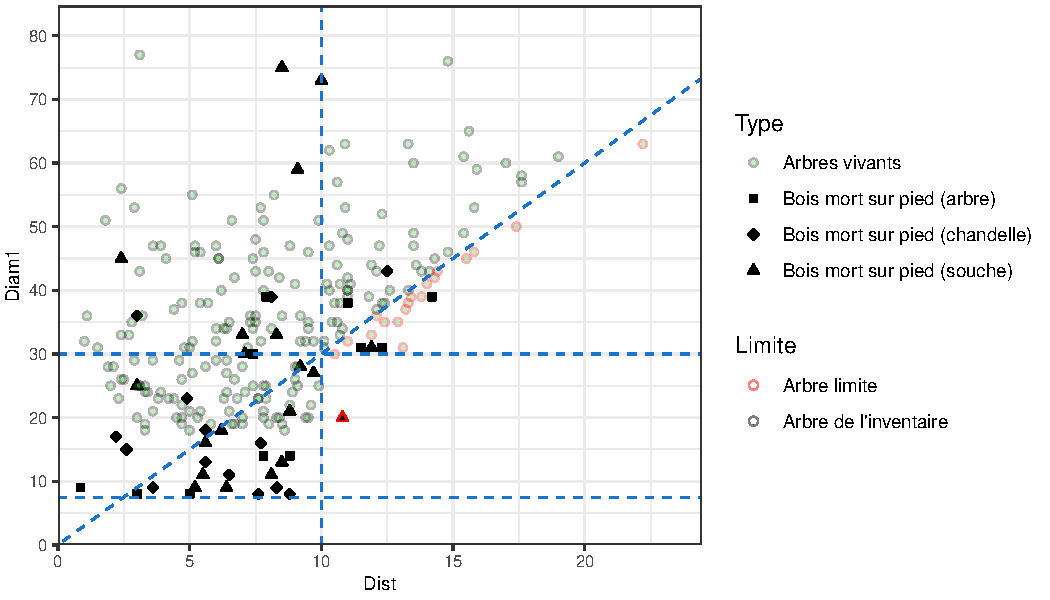
\includegraphics[width=\maxwidth]{/Users/Valentin/Travail/Outils/GitHub/PermGF-ShinyApp/out/23-Foret_Communale_dOnex/rapport_verif/figures/Arbres2-Echantillonnage_DiamDist-1} 

}

\caption[\footnotesize{Vérification de l'échantillon (\textbf{pour les arbres repérés azimut/distance du dernier inventaire)}}]{\footnotesize{Vérification de l'échantillon (\textbf{pour les arbres repérés azimut/distance du dernier inventaire)}}}\label{fig:Arbres2-Echantillonnage_DiamDist}
\end{figure}

\end{knitrout}
\FloatBarrier




























































